\section*{Question 3}
\fakesection{3}

This problem compares the window method of filter design, using various fixed windows, with the optimal Parks-McClellan method. The aim is to design a band pass FIR filter to meet the following specifications:
\begin{multicols}{2}
    \begin{itemize}
        \item Sampling frequency: $f_s=40$ kHz
        \item Stop band start: $f_1=4$ kHz
        \item Stop band end: $f_2=6$ kHz
        \item Transition width: $\Delta f=1$ kHz
        \item Stop band attenuation: $A_s=60$ dB
        \item Pass band attenuation: $A_p=1$ dB
    \end{itemize}
\end{multicols}
Using standard tables of window properties, it is possible to select an appropriate window based on theoretical stop band attenuation values\footnote{Jake Gunther, Logan, UT, USA. \textit{FIR Filter Design using the Window Method.} (Apr. 11, 2020). Accessed: Aug. 30, 2023. [Online Video]. Available: https://www.youtube.com/watch?v=2tmilbi4L0o}. However, for this exercise we will compare all four suggested windows: rectangular, Bartlett, Hann, and Blackman.

We begin by estimating an appropriate filter length using the Harris formula:
\begin{align}
    N \approx \frac{f_s}{\Delta f} \frac{A}{22} = \frac{40}{1} \frac{60}{22} = 109.\overline{09}
\end{align}
Hence, we choose an initial length of 110 taps. We now construct the ideal frequency response, $V$, which is a vector containing 0's in the stop bands and 1's in the pass band. The width of the pass band is approximated by:
\begin{align}
    L = \frac{f_2 - f_1}{f_s} \cdot N = 5.5 \text{ bins}
\end{align}
We choose to round this up to 6 bins, producing the DFT-symmetric result of Figure \ref{fig:q3_ideal_freqz}.

\begin{figure}[ht]
    \centering
    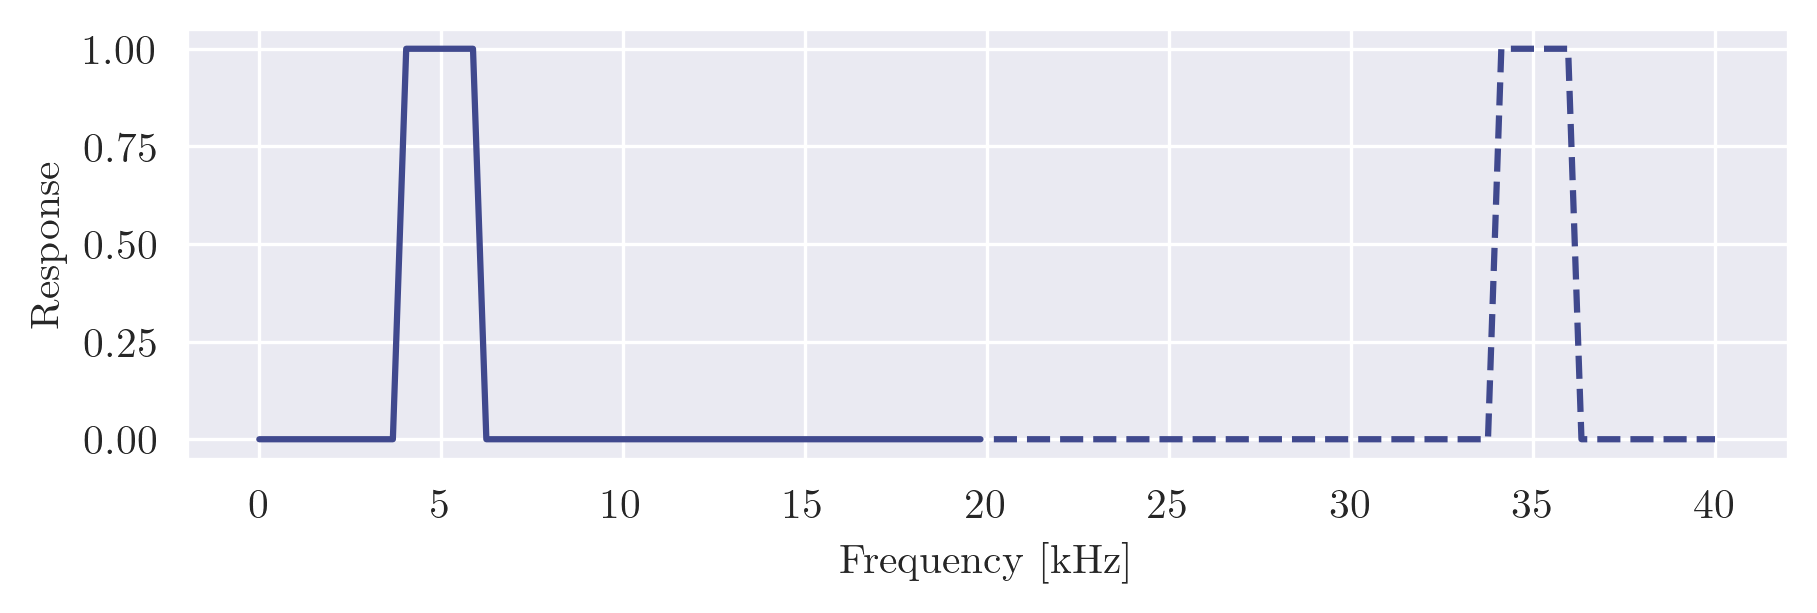
\includegraphics[width=0.7\textwidth]{images/q3_ideal_freqz.png}
    \caption{Frequency response of ideal filter, represented by vector $V$}
    \label{fig:q3_ideal_freqz}
\end{figure}

This has the associated impulse response in the time domain presented in Figure \ref{fig:q3_ideal_impz}.

\begin{figure}[ht]
    \centering
    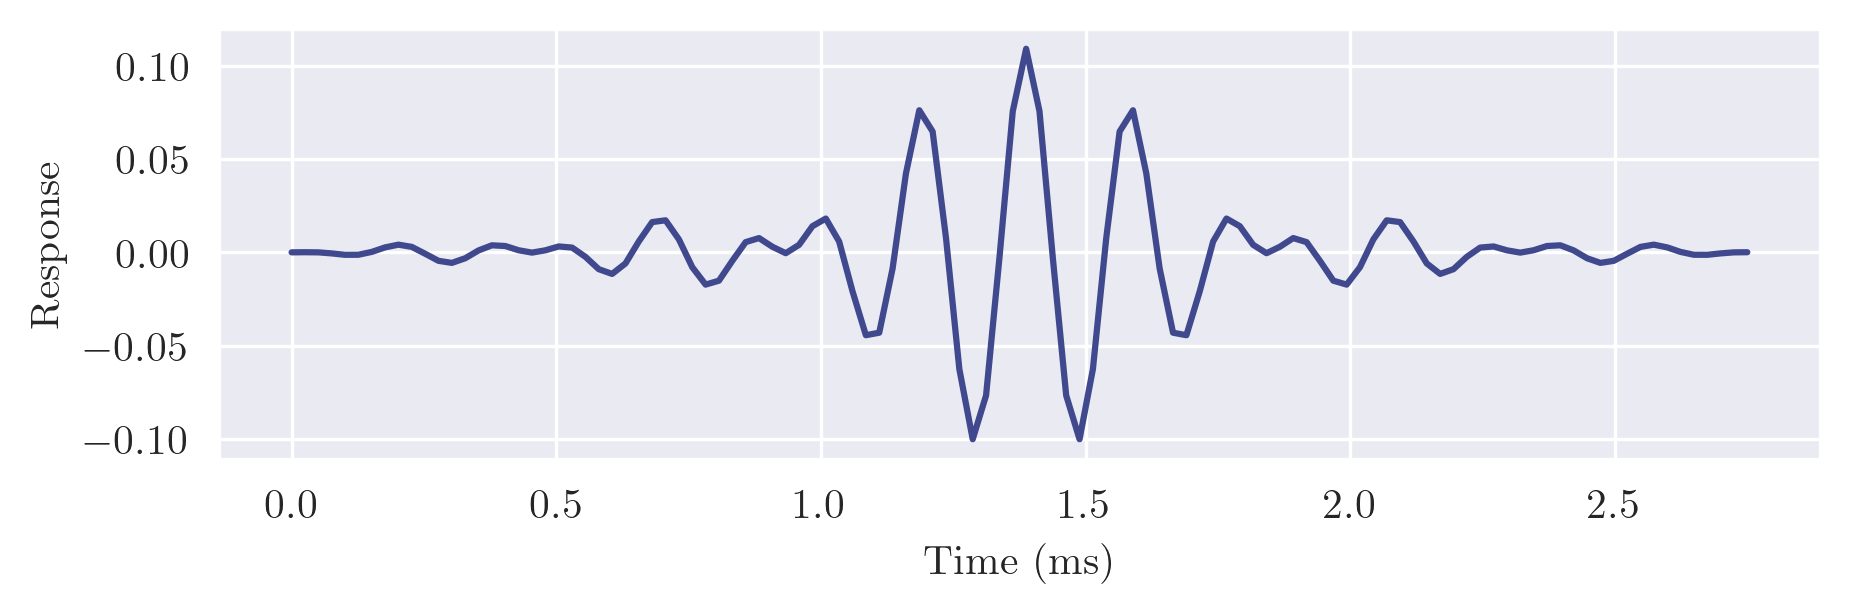
\includegraphics[width=0.7\textwidth]{images/q3_ideal_impz.png}
    \caption{Impulse response of ideal filter}
    \label{fig:q3_ideal_impz}
\end{figure}

\newpage

We multiply the ideal impulse response by each window of length $N$ to determine the frequency response of the resulting filter. The results are shown in Figure \ref{fig:q3_window_freqzs} on a decibel response scale.

\begin{figure}[ht]
    \centering
    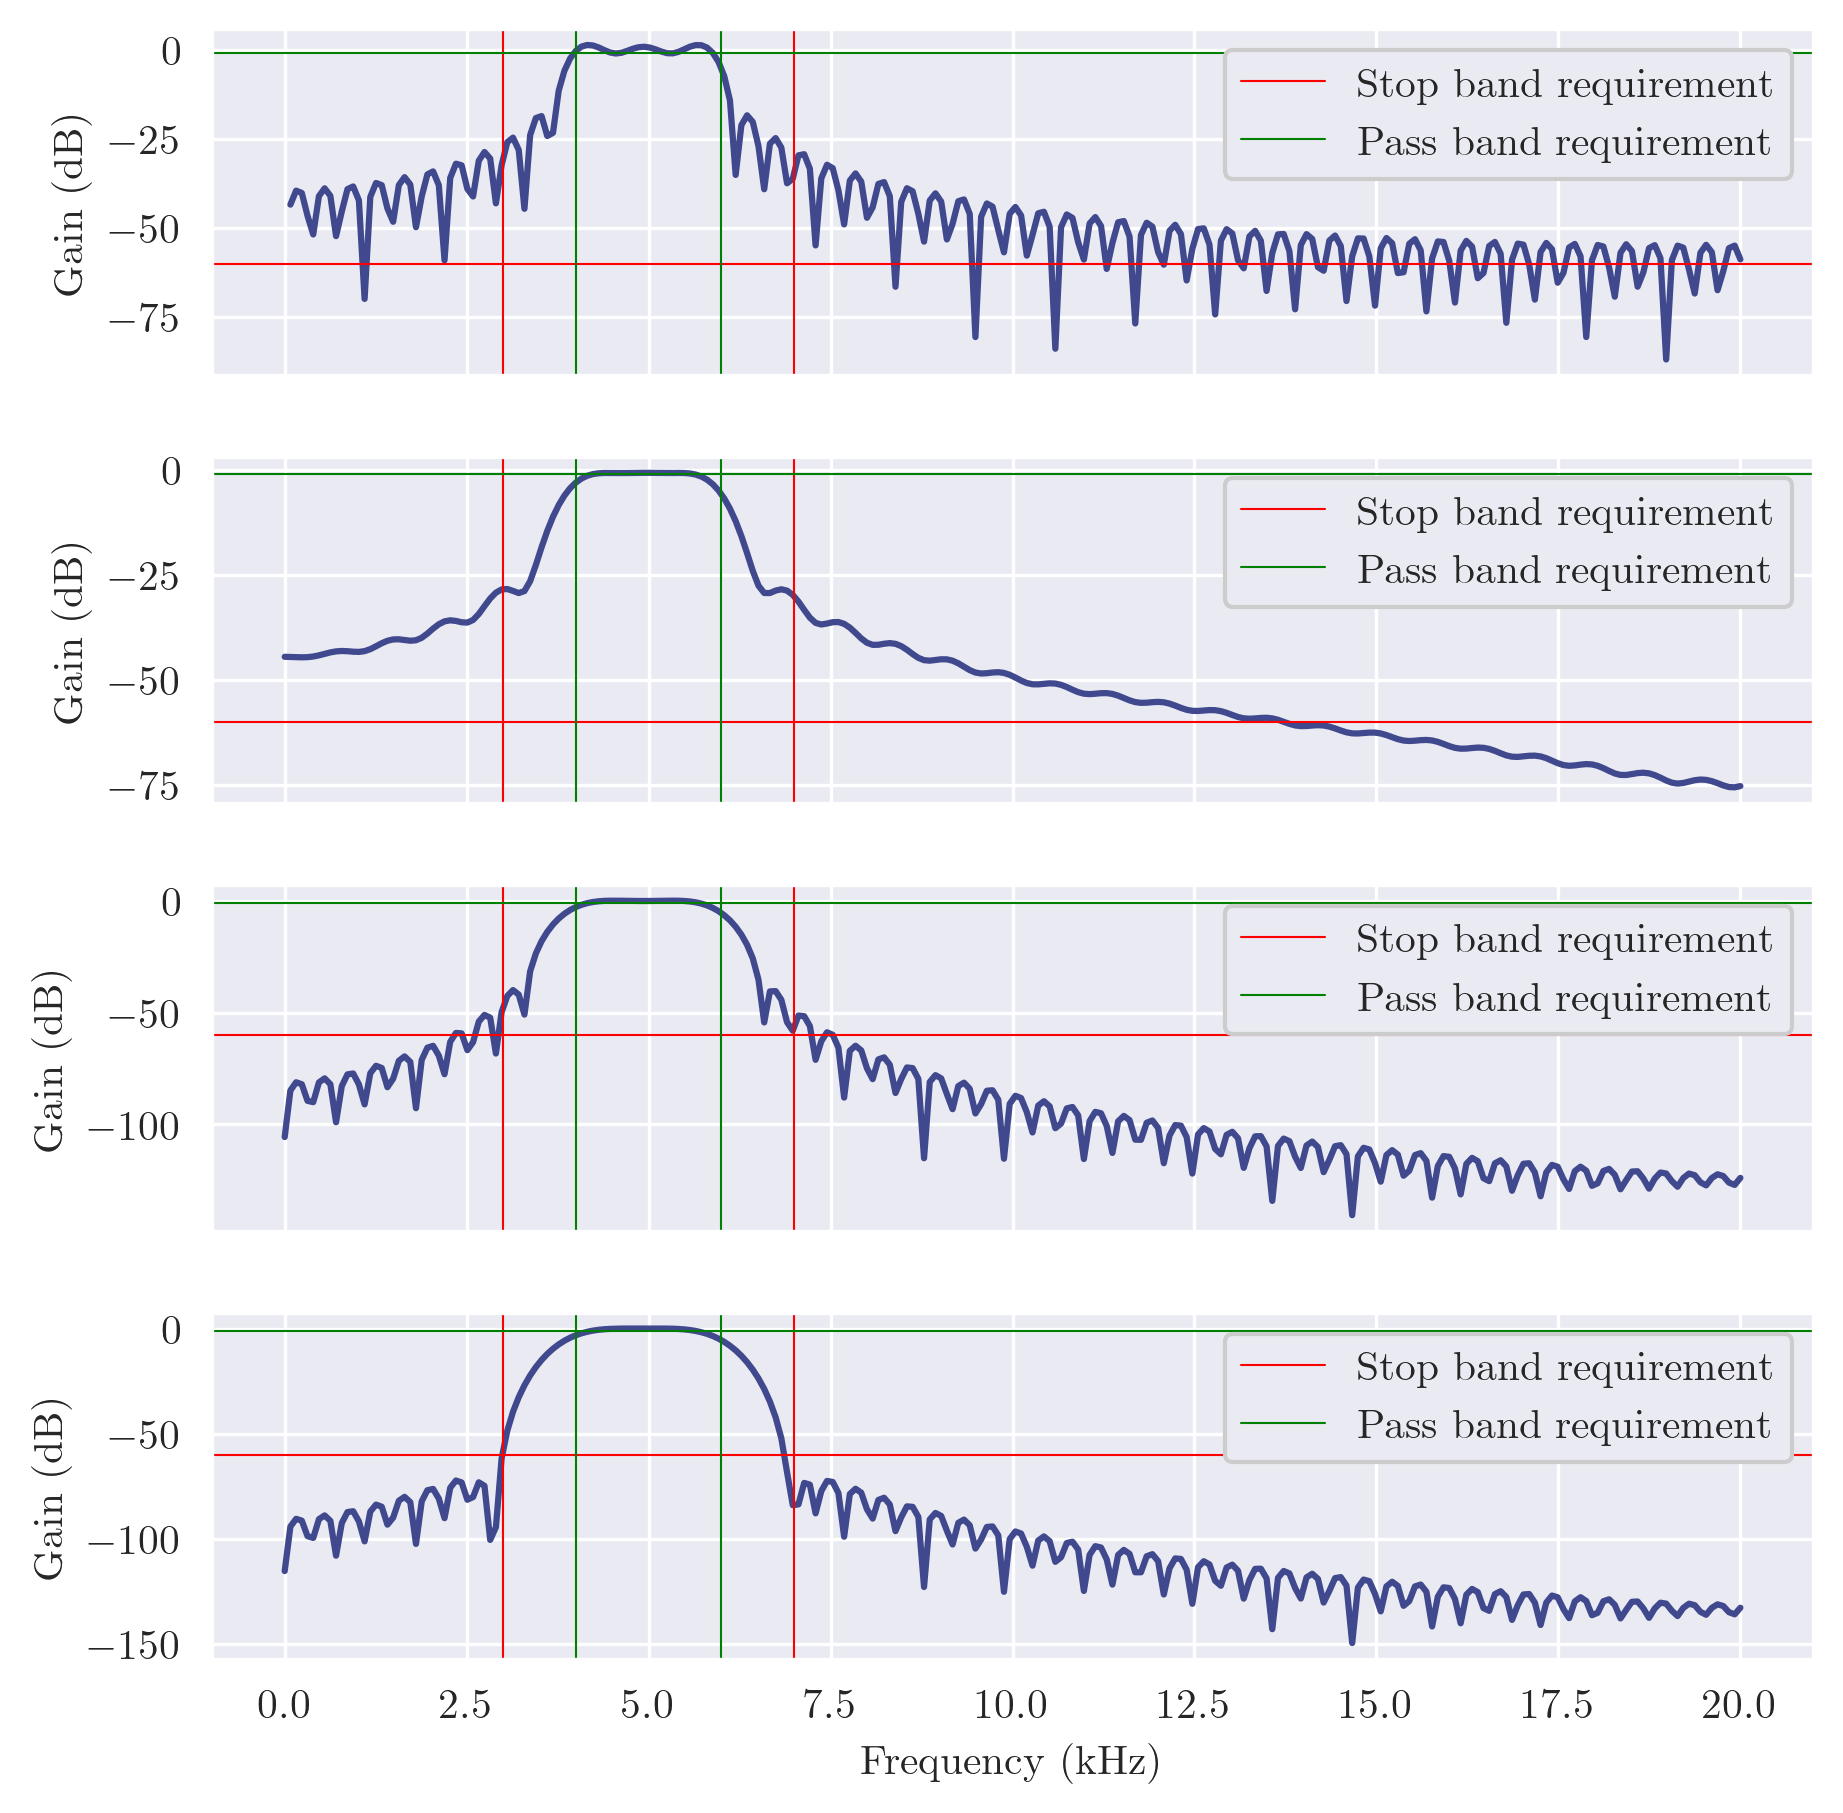
\includegraphics[width=0.8\textwidth]{images/q3_window_freqzs.png}
    \caption{Filter frequency response using various windows}
    \label{fig:q3_window_freqzs}
\end{figure}

From Figure \ref{fig:q3_window_freqzs}, only the Blackman window achieves the stop band attenuation requirement. However, the zoomed view of Figure \ref{fig:q3_zoom_1} shows that filter rolls off too quickly and does not meet the 3 dB pass band requirement at 6 kHz.

\begin{figure}[!ht]
    \centering
    \begin{subfigure}[b]{0.45\textwidth}
        \centering
        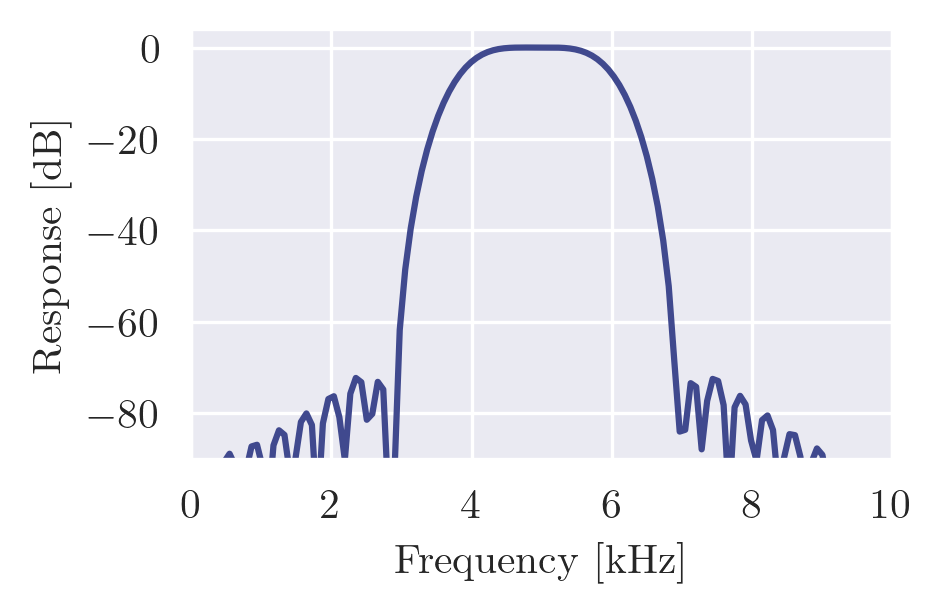
\includegraphics[width=\textwidth]{images/q3_zoom_1.png}
        \caption{Stop band specification is met}
        \label{fig:q3_zoom_0}
    \end{subfigure}
    \hfill
    \begin{subfigure}[b]{0.45\textwidth}
        \centering
        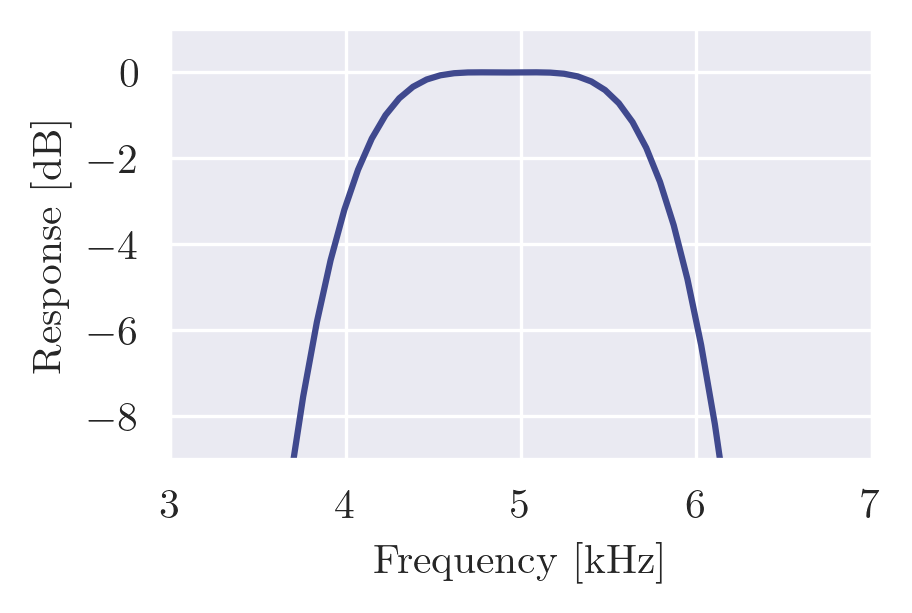
\includegraphics[width=\textwidth]{images/q3_zoom_2.png}
        \caption{Pass band specification not met}
        \label{fig:q3_zoom_1}
    \end{subfigure}
\end{figure}

As the roll-off is too fast rather than too gradual, this cannot be solved by simply increasing the length of the filter. Instead, we increase the filter length to 160 and also add one to the right side of the pass band of the ideal frequency vector, $V$.

\newpage

With these modifications, we find the Blackman-windowed filter meets all given specifications.

\begin{figure}[ht]
    \centering
    \begin{subfigure}[b]{0.45\textwidth}
        \centering
        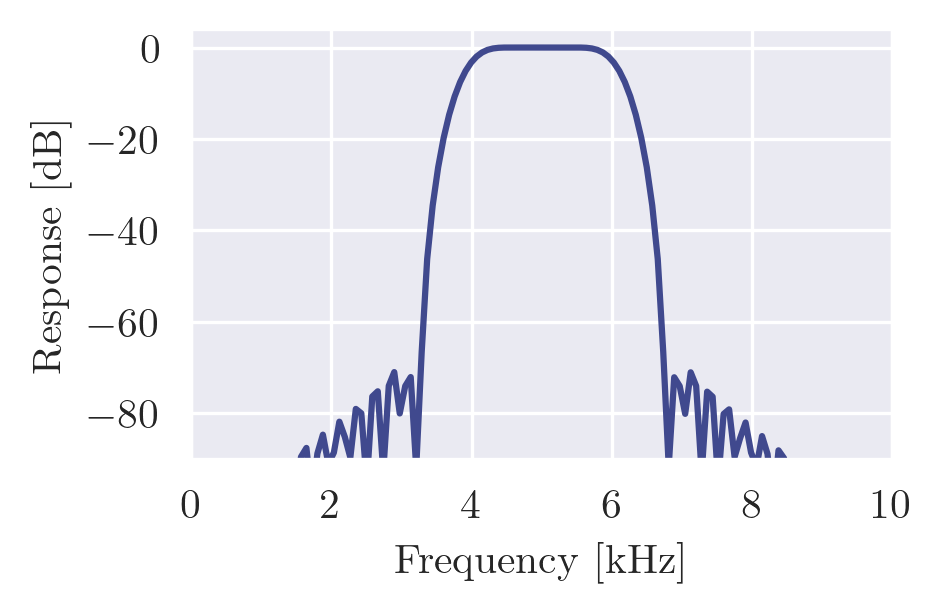
\includegraphics[width=\textwidth]{images/q3_zoom_3.png}
        \caption{Stop band specification is met}
        \label{fig:q3_zoom_3}
    \end{subfigure}
    \hfill
    \begin{subfigure}[b]{0.45\textwidth}
        \centering
        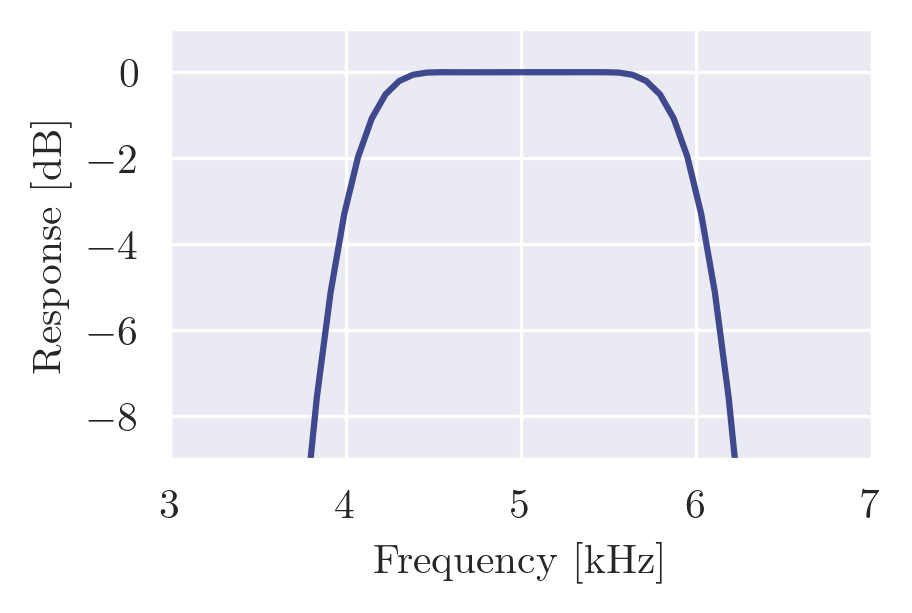
\includegraphics[width=\textwidth]{images/q3_zoom_4.png}
        \caption{Pass band specification is met}
        \label{fig:q3_zoom_4}
    \end{subfigure}
\end{figure}

We now design a filter to the same specifications using the optimal Parks-McClellan method.

\begin{figure}[ht]
    \centering
    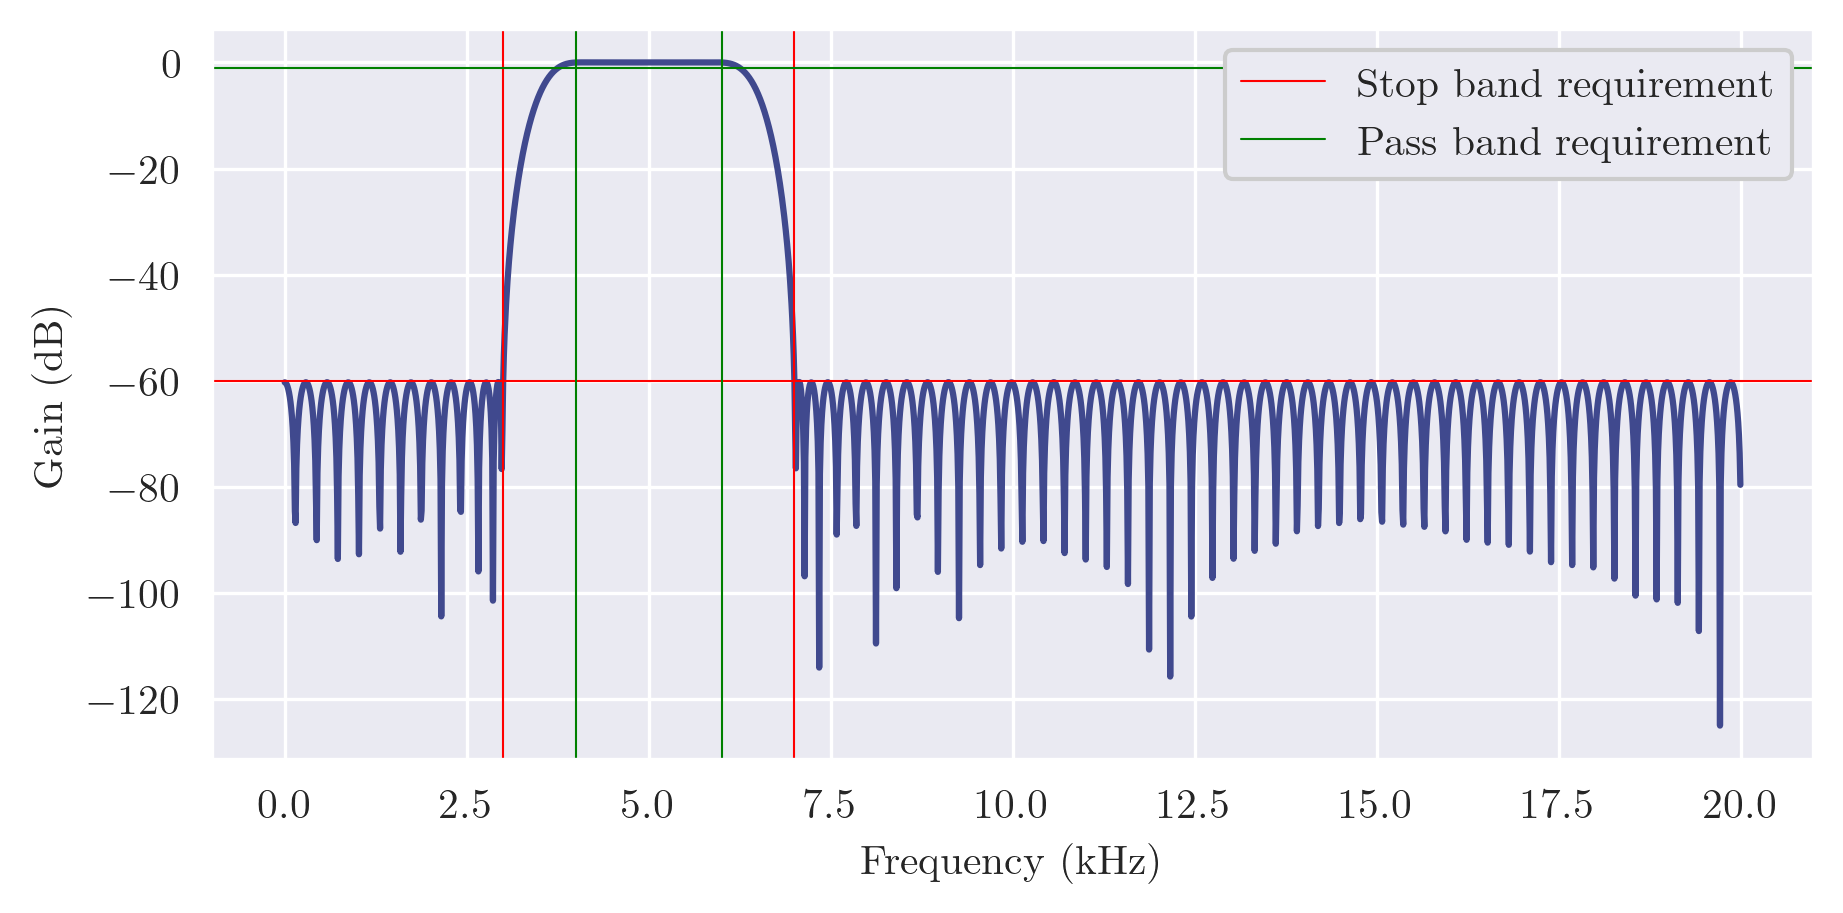
\includegraphics[width=0.9\textwidth]{images/q3_optimal_freqz.png}
    \caption{An optimal filter designed using the Parks-McClellan method}
    \label{fig:q3_optimal_freqz}
\end{figure}

This filter was implemented using the \texttt{scipy.signal.remez} method. Starting from the final Blackman-windowed filter length of 160, the number of taps in the optimal filter was reduced until just meeting the requirements. The final filter shown in Figure \ref{fig:q3_optimal_freqz} has 140 taps.
